%%%%% Document Setup %%%%%%%%

\documentclass[10pt, twocolumn]{revtex4}    % Font size (10,11 or 12pt) and column number (one or two).

\usepackage{times}                          % Times New Roman font type

\usepackage[a4paper, left=1.85cm, right=1.85cm,
 top=1.85cm, bottom=1.85cm]{geometry}       % Defines paper size and margin length

\usepackage[font=small,
labelfont=bf]{caption}                      % Defines caption font size as 9pt and caption title bolded
\captionsetup{justification=raggedright, singlelinecheck=false}

\usepackage{mathtools,amssymb}
\usepackage{graphics,graphicx,epsfig,ulem}	% Makes sure all graphics works
\usepackage{amsmath} 						% Adds mathematical features for equations
\usepackage{siunitx}
\usepackage{textcomp}
\usepackage{enumitem}
\usepackage{bm}
\usepackage{lipsum}
\usepackage[toc,page]{appendix}
\usepackage{booktabs}
\usepackage{rotating}
\usepackage{siunitx}
\usepackage{multirow}
\usepackage{ulem}
\usepackage{array}
\newcolumntype{L}[1]{>{\raggedright\arraybackslash}p{#1}}

\usepackage{etoolbox}                       % Customise date to preferred format
\makeatletter
\patchcmd{\frontmatter@RRAP@format}{(}{}{}{}
\patchcmd{\frontmatter@RRAP@format}{)}{}{}{}
\renewcommand\Dated@name{}
\newcommand{\rom}[1]{\uppercase\expandafter{\romannumeral #1\relax}}
\makeatother

%\usepackage[flushleft]{threeparttable}

\usepackage{fancyhdr}

\pagestyle{fancy}                           % Insert header
\renewcommand{\headrulewidth}{0pt}
\lhead{P. Einarsson Nielsen}                          % Your name
\rhead{Density Dependence of the Excess Energy and Pressure of a System of Lennard-Jones Particles}           % Your report title               

\def\bibsection{\section*{References}}        % Position refernce section correctly


\AtBeginDocument{
	\heavyrulewidth=.08em
	\lightrulewidth=.05em
	\cmidrulewidth=.03em
	\belowrulesep=.65ex
	\belowbottomsep=0pt
	\aboverulesep=.4ex
	\abovetopsep=0pt
	\cmidrulesep=\doublerulesep
	\cmidrulekern=.5em
	\defaultaddspace=.5em
}
\renewcommand{\arraystretch}{1.2}


%%%%% Document %%%%%
\begin{document}                     


\title{Density Dependence of the Excess Energy and Pressure of a System of Lennard-Jones Particles} 
\date{Submitted: \today{}}
\author{P. Einarsson Nielsen}
\affiliation{\normalfont PHYS3561: Computing Project}

\begin{abstract}
	The Monte Carlo method is applied to evaluate the radial distribution function and thus compute excess energy per particle and pressure for systems of three-dimensional particles interacting via the Lennard-Jones potential in an NVT ensemble. The Lennard-Jones parameters are those of argon. Systems were simulated for twenty-four reduced densities between \num{0.05} and \num{1.50} along reduced temperatures \num{0.75}, \num{1.00}, \num{1.25}, \num{1.50}. Along the two higher isotherms we find the excess energy per particle to be slightly lower than literature values across all densities but in otherwise good agreement. This is likely due to an approximation made when computing the excess energy. The shape of the density dependence of the excess pressure is consistent with literature with some inconsistencies in scale, likely indicating a small error in the evaluation of the radial distribution function which could also explain erratic behaviour observed in the excess energy at low densities not replicated in literature. Radial distribution functions typical of vapour, liquid and solid states are presented.
	
	
	

\end{abstract}

\maketitle
\thispagestyle{plain} % produces page number for front page



\section{Introduction} \label{s:intro}

The Monte Carlo (MC) method of calculating thermodynamic properties has been well established since originally developed and applied on hard disks \cite{MC}. It has had wide reaching impacts on sectors ranging from its intended purpose of thermodynamic simulations to computational biology and finance. The Monte Carlo method allows for computer simulations of systems; often under conditions which would be very complex or costly to perform experimentally. This makes it a very versatile tool for obtaining essentially microscopically exact results on various systems. Computer simulations also allow us to wholly determine the method by which particles interact \cite{CompSimLiq}.

One of the effects that is much more straight forward to investigate by computer simulations than by physical experiments is phase transitions which are driven by entropy. Somewhat counter-intuitively, increasing the entropy, which is often considered a measure of the disorder in a system, can actually incite transitions from vapour to liquid to solid states in some systems. This is the method by which phase transition presented in this report occur \cite{Frenkel, Hansen2}.

In this work we investigate three-dimensional spheres interacting by the Lennard-Jones (LJ) potential in an NVT ensemble, where the number of particles, volume and temperature are kept constant. Throughout this work we will use reduced units for distances, temperatures and densities ($\rho{}=N/V$ is number density):
\begin{displaymath}
r^{*} = r/\sigma{},\quad{}
T^{*} = k_\text{B}T/\epsilon{},\quad{}
\rho{}^{*} = \rho{}\sigma{}^{3} = (N/V)\sigma{}^{3}
\end{displaymath}
%\begin{displaymath}
%T^{*} = k_\text{B}T/\epsilon{},
%\end{displaymath}
%\begin{displaymath}
%\rho{}^{*} = \rho{}\sigma{}^{3} = (N/V)\sigma{}^{3}.
%\end{displaymath}
where $\sigma{}$ is the finite distance at which the LJ potential evaluates to zero and $\epsilon{}$ is the depth of the potential well. When these parameters are fitted to experimental data, the LJ potential can accurately describe the interactions between particles in certain systems, particularly for atoms of noble gases \cite{SimpleLiquids}. MC simulations of particles interacting with the LJ are also often performed for their own merit, with the parameters $\sigma=\num{3.4e10}$m and $\epsilon=\num{1.65e21}$J corresponding to argon taken by convention \cite{WoodParker}. We use these parameters in our simulations.
In its reduced form, the LJ potential between two particles can be expressed as
\begin{equation}
U_{LJ}(r^{*}) = 4\left[\left(\frac{1}{r^{*}}\right)^{12}-\left(\frac{1}{r^{*}}\right)^{6}\right]
\end{equation}
where $r^{*}$ is the separation of the two particles.
We perform these simulations for a number of initial configurations, varying the density and temperature of the system.


\section{Methodology} \label{s:methods}
We simulated systems of $N=1000$ particles interacting with the LJ potential. The particles were initialised in a face-centred cubic (FCC) lattice within a cubic container of volume $V$. Conventional boundary conditions, where a particle which moves beyond the boundary of its container is moved to the opposite side, were applied.
MC involves applying a random Cartesian move to each particle in turn, described by
\begin{displaymath}
\Delta{}\bar{s} = d\left(\bar{\xi}-0.5\right)
\end{displaymath}
where $\bar{s}$ and $\bar{\xi}$ are three-vectors containing the move and random numbers between 0 and 1 respectively and $d$ is the maximum displacement.
The change in total potential energy of the new configuration is calculated under the assumption of additivity of pair potentials, i.e. that the total potential energy can be expressed by the sum of the LJ potential between every particle in the system. As we keep the particle number constant and vary the container size to achieve different densities, the LJ potential is truncated at different distances at different densities, although always half the container length. In practise this leads to truncation at $r^{*}=10.8, 4.4$ for systems of densities $\rho{}^{*}=0.1, 1.5$ respectively, which gives more accurate total potentials than the $r^{*}=3$ truncation scheme used by some workers \cite{NIST}.
A move was accepted if it resulted in a decrease in the total potential energy of the system. If not, the move was accepted with a probability proportional to the Boltzmann factor of the resulting state,
\begin{displaymath}
\exp{\frac{\Delta{}U_\text{LJ}}{k_\text{B}T}}.
\end{displaymath}
where $\Delta{}U, k_\text{B}, T$ are the change in potential energy, Boltzmann constant and system temperature respectively.
This over-weights rarer configurations and is known as importance sampling. At equilibrium, each move is reversible by a move in the opposite direction and, as such, this algorithm satisfies detail balance \cite{CompSimLiq}.
The system was equilibrated over a number, $N_\text{equil}$, of moves such that the initial FCC structure is not present. The maximum displacement, $d$, is adjusted periodically during this equilibration such that the 30-50\% of moves were accepted.
The system was then evolved over further number, $N_\text{evolve}$, of moves and its configuration sampled periodically. The radial distribution function (RDF), $g(r)$, was then calculated and averaged over each particle. The RDF tells us the probability, relative to the ideal gas case, of finding a molecule at a given distance from a reference particle and can be expressed as
\begin{displaymath}
g(r) = \frac{n(r)}{n_\text{ideal}(r)}
\end{displaymath}
where $n_\text{ideal} = \rho{}4\pi{}r^{2}\Delta{}r$, $n(r)$ is the number of particles within a shell of thickness $\Delta{}r$ at a distance $r$, $\rho{}$ is the number density of the system.

System properties relating to its configuration can be computed from $g(r)$. We compute the excess internal energy per particle by the energy equation \ref{eq:energy} and the excess pressure of the system by the virial equation \ref{eq:pressure} \cite{WoodParker, Johnson}.
\begin{equation}
u^{*} = 2\pi{}\rho{}\int_{0}^{\infty}U_\text{LJ}(r^{*})g(r^{*})(r^{*})^{2}dr^{*}
\label{eq:energy}
\end{equation}
\begin{equation}
p^{*} = P - \rho{}k_\text{B}T = - \frac{2\pi}{3}\rho{}^{2} \int_{0}^{\infty}\frac{U_\text{LJ}(r^{*})}{dr^{*}}g(r^{*})(r^{*})^{3}dr^{*}
\label{eq:pressure}
\end{equation}
In practise the integrals in equations \ref{eq:energy} and \ref{eq:pressure} were approximated as Riemann sums with $dr^{*} \rightarrow{} \Delta{}r^{*} = 0.02$, calculated up to a maximum distance of $r_\text{max}^{*}=6$. The effect of this approximation is discussed in section \ref{ss:numerical}.
With the assumption that at a sufficiently large $r^{*}$ every system looks homogeneous, i.e. that $g(r^{*})$ converges to unity at large $r^{*}$, we can account for our truncated LJ interaction using standard long range corrections. Johnson et al give analytic expressions for these in equations (2) and (3) in \cite{Johnson}.

Each system discussed within was equilibrated over $N_\text{equil}=\num{2e7}$ moves, evolved over $N_\text{evolve}=\num{2e7}$ moves and the configuration sampled every \num{2000} moves. Each simulation required approximately 30 hours of computation time. Multiple simulations were run in parallel on the CPU partition on Computer Science Department's NVIDIA Cuda Cluster at Durham University.



\section{Results \& Discussion} \label{s:results}
\subsection{Thermodynamic quantities} \label{ss:thermodynamics}
A graph showing the excess energy per particle, $u^{*}$, as a function of density, $\rho{}^{*}$, is shown in figure \ref{fig:excessEnergy}. Along the isotherms $T^{*} = 1.25, 1.50$ the configuration energy decreases visually linearly until a density in the neighbourhood of \num{0.6} at which point the gradient of the lines begin to increase with, with $u^{*}$ reaching a local minima at $\rho^{*}=1.0\pm{}0.1$ before increasing rapidly at higher densities. The excess energy of a particle quantifies how much of its energy is due to its configuration. At very low densities we observe $u^{*}$ to tend towards zero since in this regime the particles are separated by relatively large distances and the LJ potential is thus weak. When $u^{*}=0$ the energy of the particles would be that of ideal particles and thus we say that the energy of the systems become more ideal-like the smaller their densities are. At larger densities the system deviates from the ideal case. The large increase in $u^{*}$ with density beyond $\rho{}=1.0$ implies that the particle interactions and configuration provide a significant proportion of the energy of the system at these densities.
At temperatures $T^{*}=0.75, 1.00$, $u^{*}$ is observed to display erratic behaviour at small densities. This behaviour is more prominent at the lower of the two temperatures. In both cases, $u^{*}$ appears to converge to a shape similar to that of temperatures $T^{*}=1.25, 1.50$ at densities around \num{0.6} although this happens at a smaller density at $T^{*}=0.75$ than it does at $T^{*}=1.00$ - all four isotherms show similar characteristics beyond these densities. $u^{*}$ decreases smoothly until they reach the local minima at $\rho^{*}=1.0\pm{}0.1$ beyond which their variation with density is no longer smooth. In section \ref{ss:numerical} we will argue that this is most likely due to insufficient numerical convergence of results in this high-density regime.
In general, $u^{*}$ at higher temperatures is observed to lie above that of lower temperatures, implying that lower densities, less than approximately \num{1}, particle interactions have a smaller effect on the energy of a system at lower densities while at higher densities, greater than \num{1}, interactions have a larger effect which increases with density on the system energy.

A graph showing the excess pressure, $p^{*}$, as a function of density, $\rho{}^{*}$, is shown in figure \ref{fig:excessPressure}. At each isotherm, $p^{*}$ is observed to initially decrease slowly with increasing $\rho^{*}$ before reaching some local minima and then rising rapidly, a shape known as a van der Waals loop. These minima are located at densities of $0.7\pm{}0.1, 0.60\pm{}0.03, 0.55\pm{}0.05, 0.50\pm{}0.05$ for increasing isotherms where the uncertainty is taken to be the larger of the two differences in density to the nearest result. The results of Hansen \& Verlet for a homogenised LJ fluid at isotherms $T^{*}=0.75, 1.15$ contain similar van der Waals loops \cite{HansenVerlet1}. Their results also show that the density of the minima decreases with increasing temperature as is typical for isotherms of pressure-density data. The minima of their isotherm at $T^{*}=0.75$ is determined to be $6.8\pm{0.3}$, in close agreement to our value at the same temperature.
At very low densities we see that $p^{*}$ tends to zero which corresponds to the case of an ideal gas by similar arguments as for $u^{*}$.
Similar to $u^{*}$, our $p^{*}$ data can be split into three categories, grouped by density. At low densities less than about \num{0.6} the behaviour of the lower two isotherms is somewhat erratic. Between densities of about \num{0.6} and \num{1.0} similar smooth increases in $p^{*}$ are seen for all isotherms. For densities greater than \num{1.0}, $p^{*}$ continues to increase with density but this is no longer smooth. Again, this is most likely attributed to non-converged radial distribution functions at high densities.
In general, $p^{*}$ at higher temperatures is observed to lie above that of lower temperatures. As $p^{*}$ is the deviation of the simulated pressure from that predicted by the ideal-gas law this would imply that at lower densities, where $p^{*}$ is negative, a higher temperature system is more ideal-like than a system at a lower temperature while the opposite is true at higher densities, where $p^{*}$ is positive.

\begin{figure}
	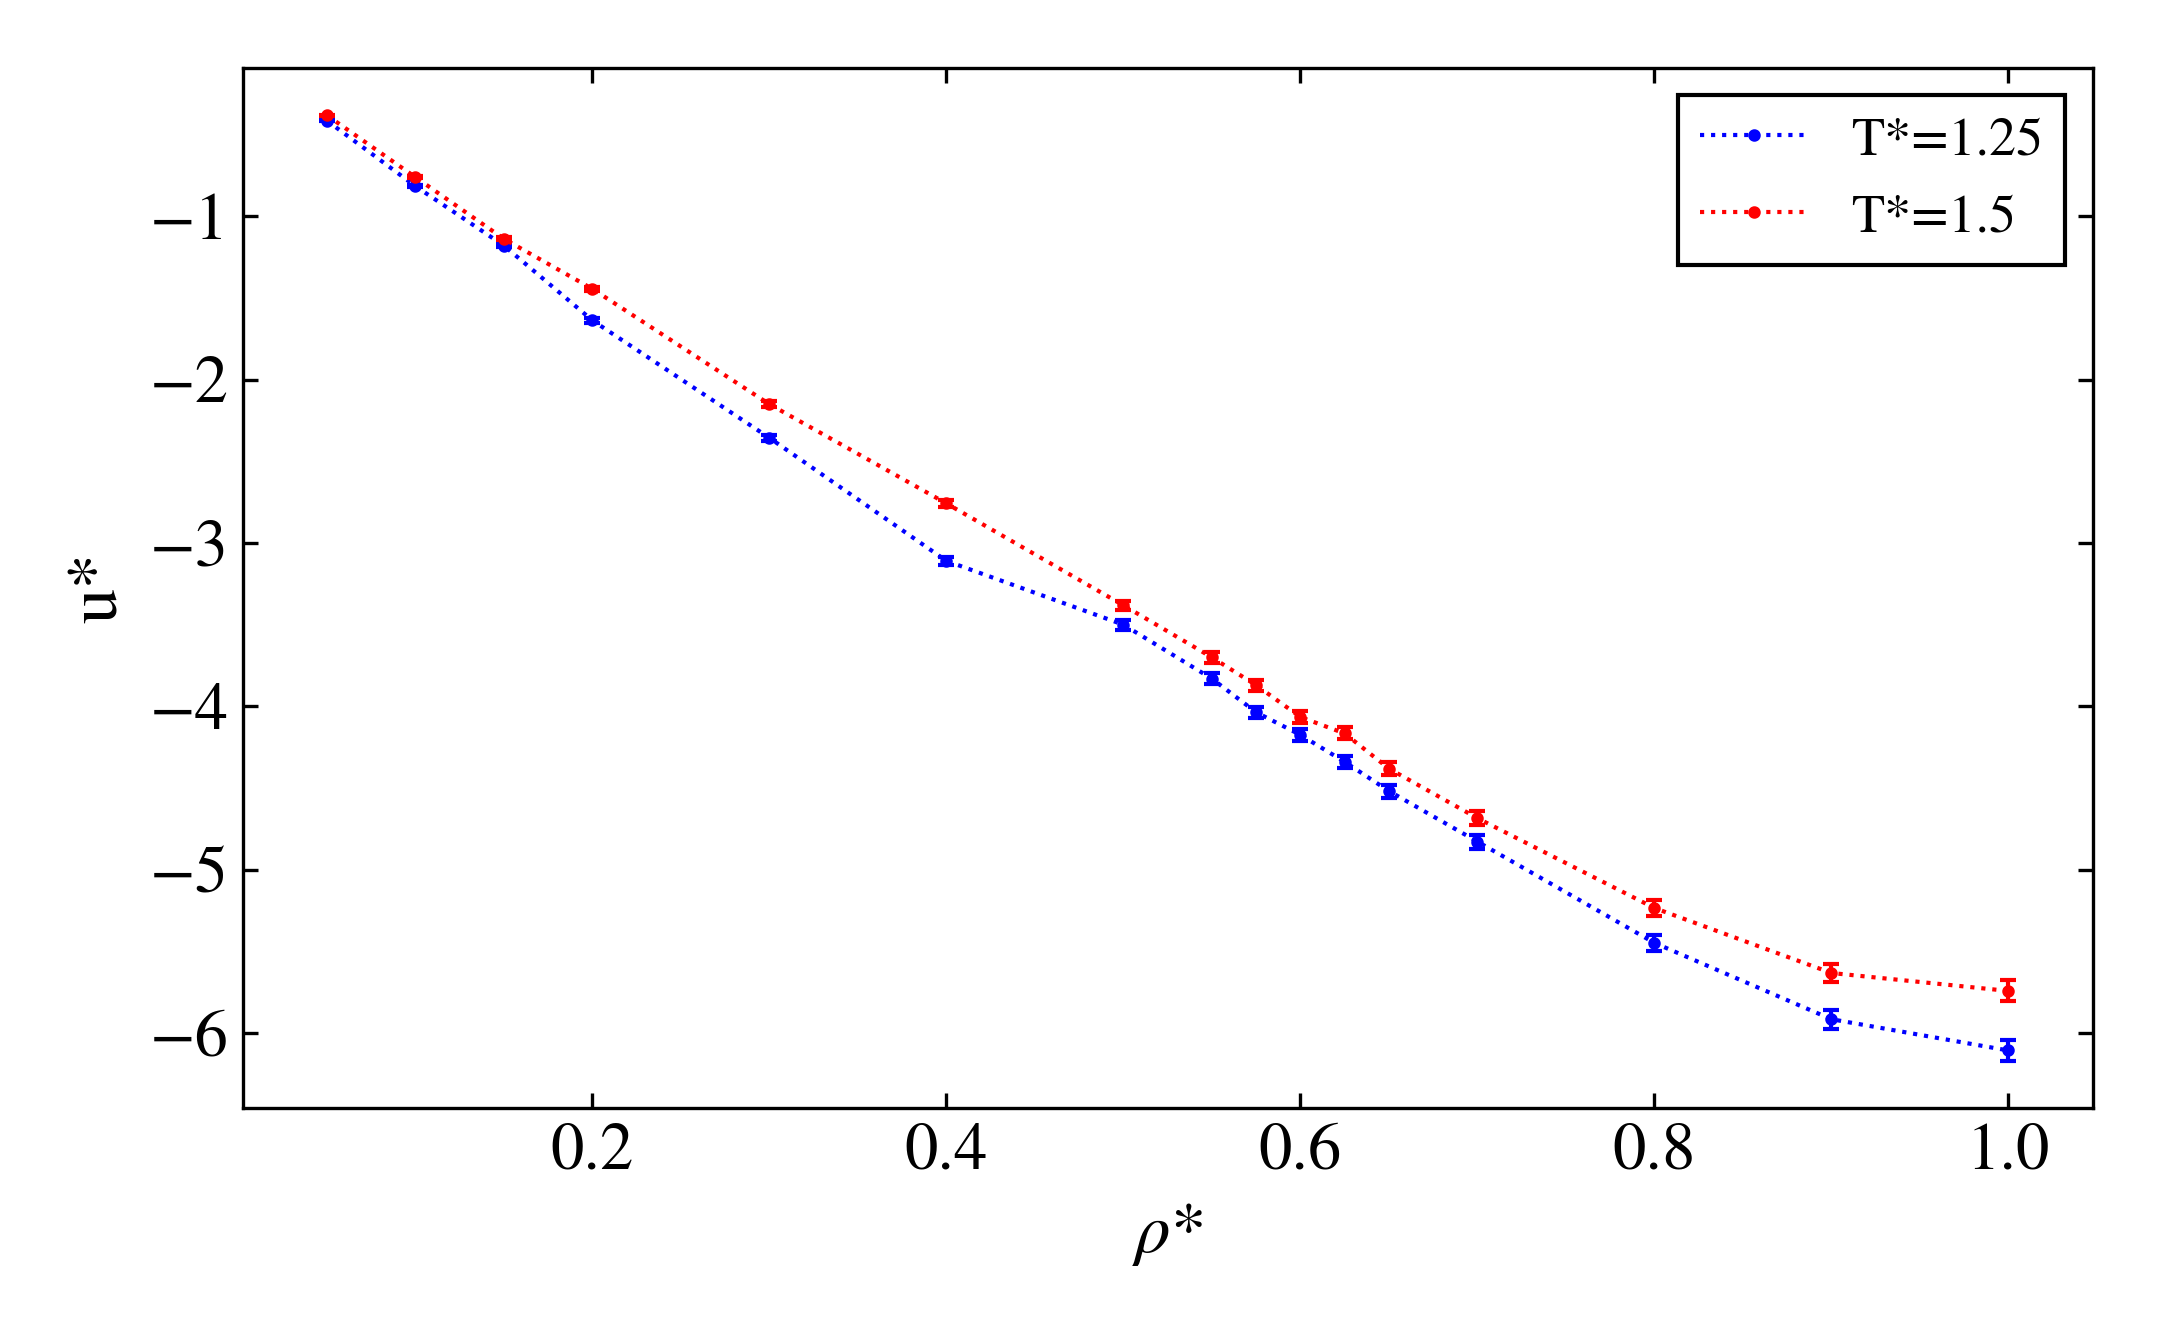
\includegraphics[width=\linewidth]{figures/excessEnergyPressure/excessEnergy.png}
	\caption{MC results for the excess energy per particle, $u^{*}$, against density, $\rho{}^{*}$ along four isotherms $T^{*}=0.75, 1.00, 1.25, 1.50$, each represented by a colour ranging from blue to red. Error bars show the standard error of the mean \cite{errors}. Dotted lines have been added to guide the eye.}
	\label{fig:excessEnergy}
\end{figure}
	
\begin{figure}
	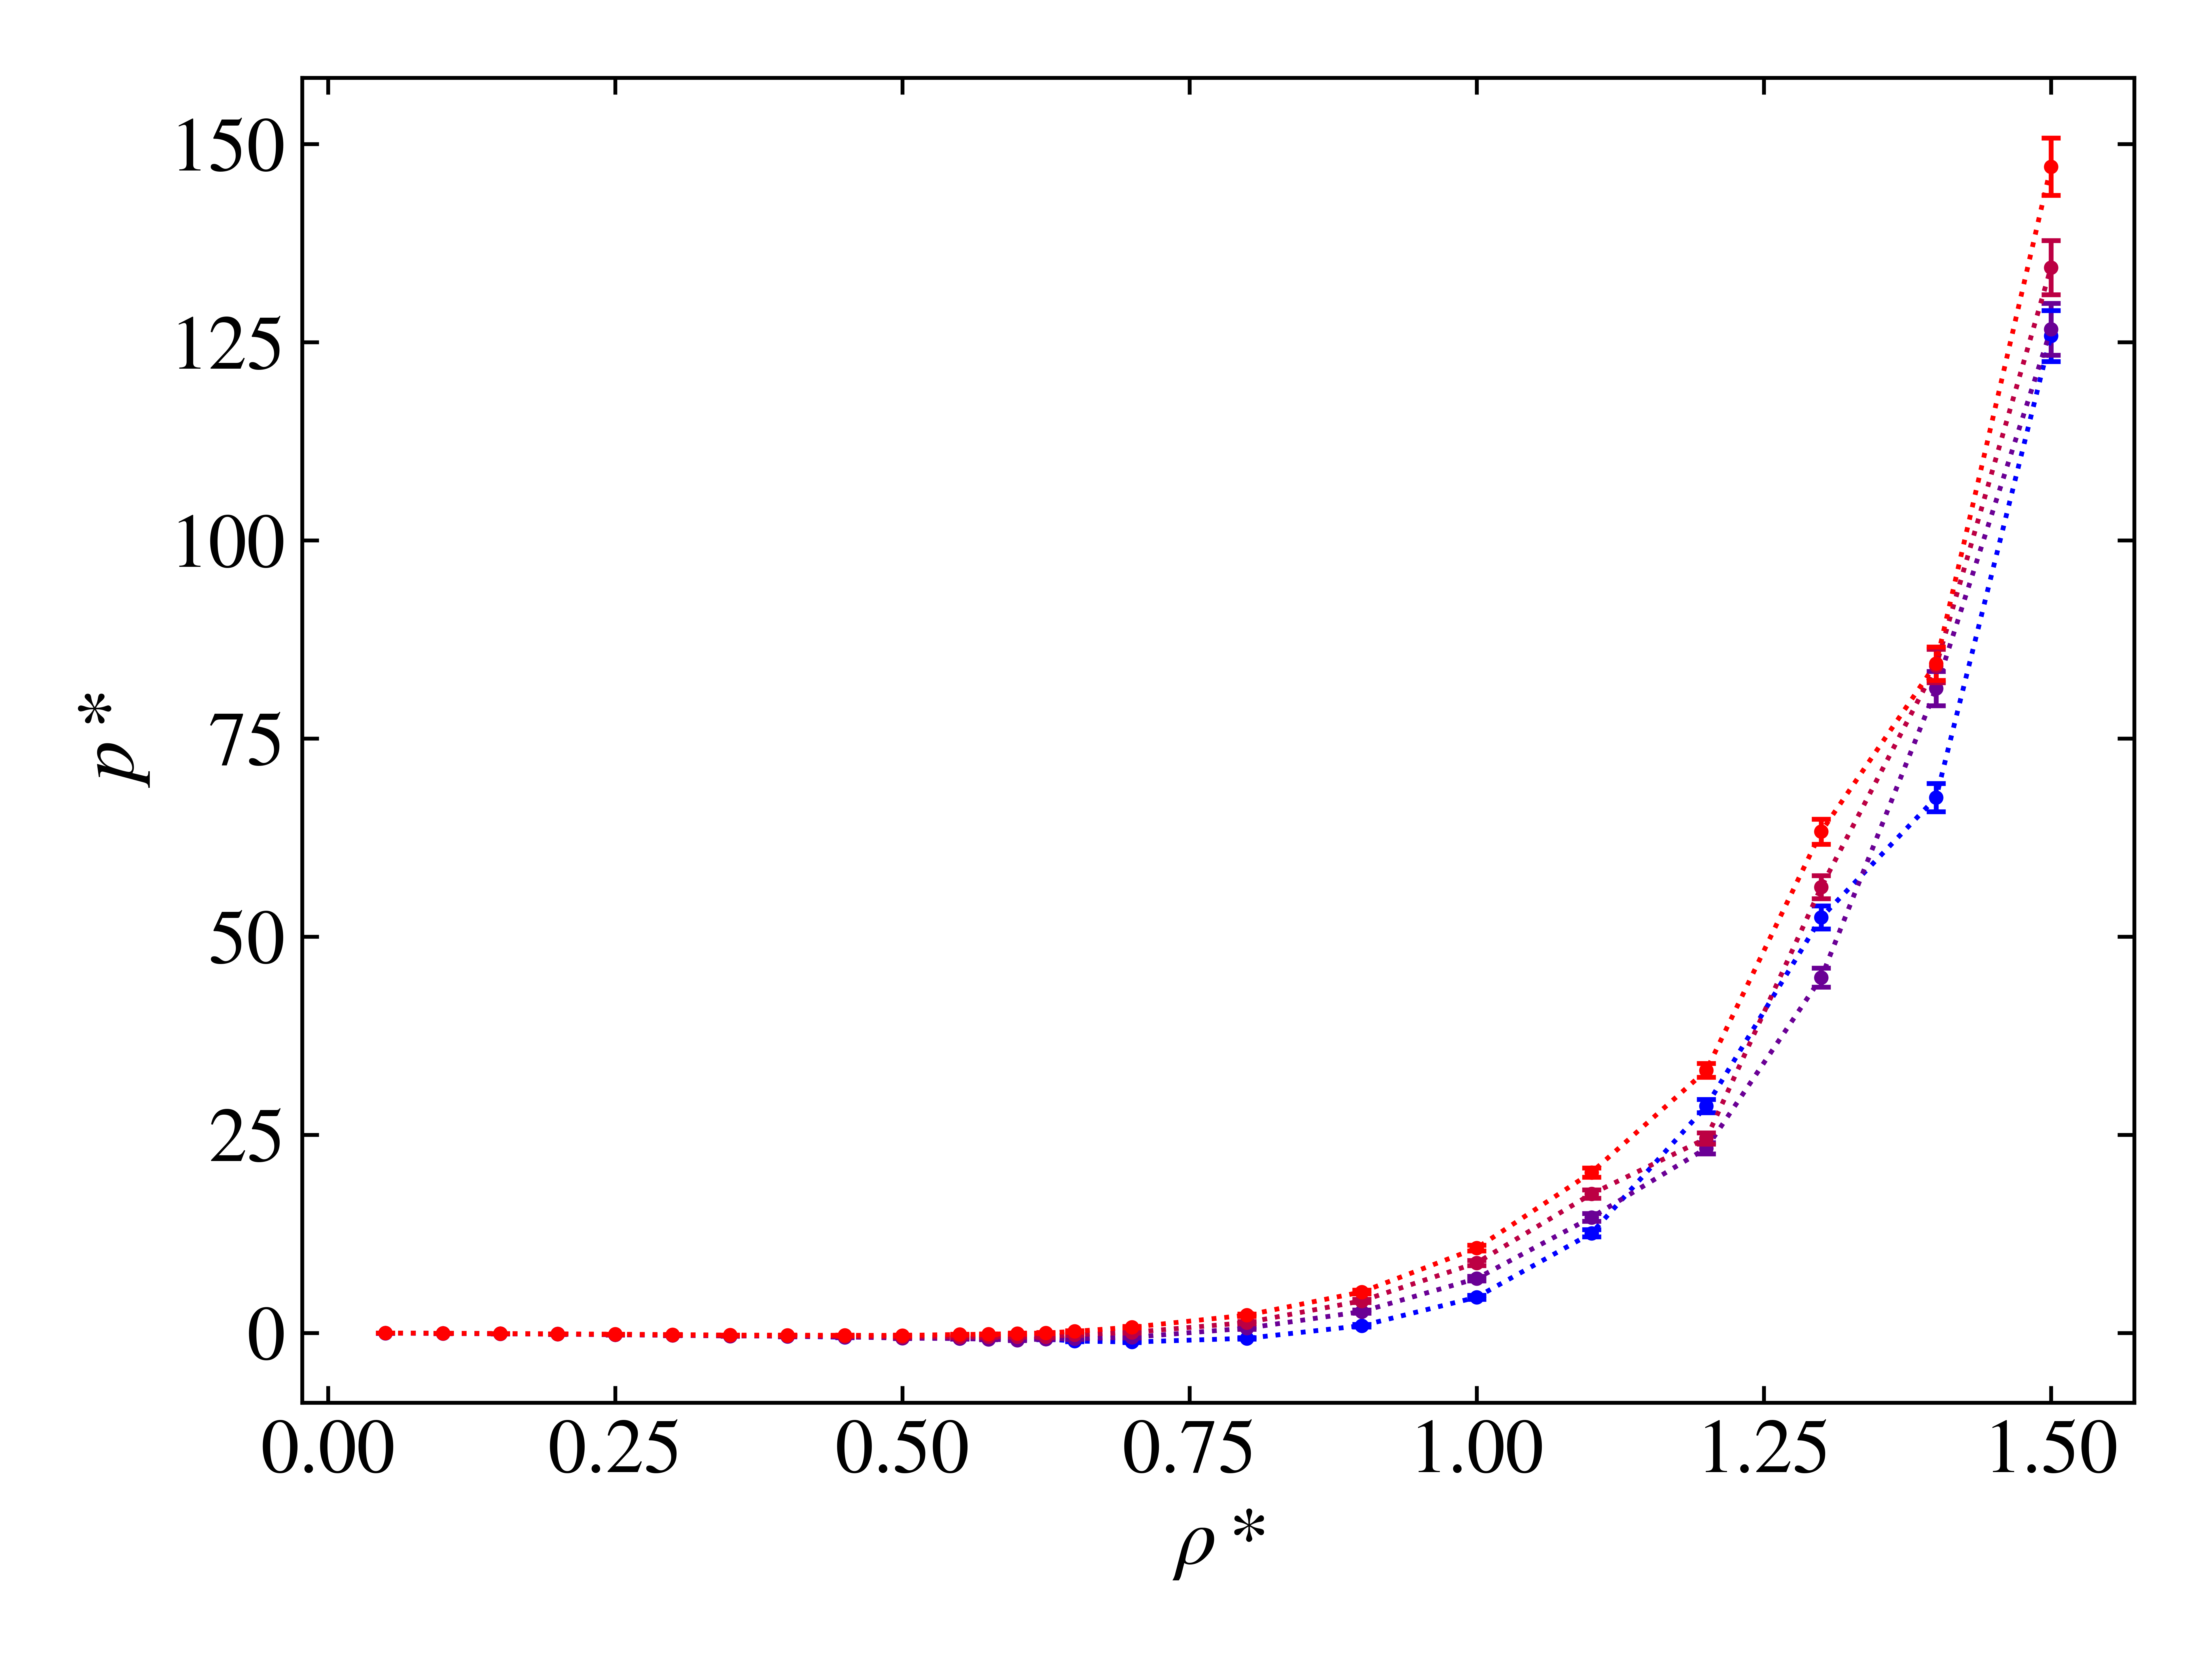
\includegraphics[width=\linewidth]{figures/excessEnergyPressure/excessPressure.png}
	\caption{MC results for the excess pressure, $p^{*}$, against density, $\rho{}^{*}$ along four isotherms $T^{*}=0.75, 1.00, 1.25, 1.50$, each represented by a colour ranging from blue to red. An inset axis shows $p^{*}$ in the density range \num{0} to \num{0.9}. Error bars show the standard error of the mean. Error bars are omitted for the middle two isotherms for visual clarity. Dotted lines have been added to guide the eye.}
	\label{fig:excessPressure}
\end{figure}

In the range of densities investigated here we expect our systems to show examples of three different states: vapour, liquid and solid. We make no attempt at identifying the critical parameters of $T^{*}$ and $\rho{}^{*}$ at which transitions between the states occur. Other workers have identified these parameters for various systems by MC methods, molecular dynamics and theoretical approaches \cite{Ree}. Wood \& Parker found a vapour-to-liquid transition to occur in the region of $\rho{}^{*}=0.40$ and a liquid-to-solid transition in the region of $\rho{}^{*}=1.10$ for MC systems on isotherms $T^{*}=2.74$ \cite{WoodParker}. Guided by these values we show in figure \ref{fig:RDFs} the radial distribution functions of systems of densities $\rho{}^{*}=0.1, 0.8, 1.5$, corresponding to a vapour, liquid and solid state respectively, at a temperature $T^{*}=1.5$. What follows is a qualitative discussion about the features of the radial distribution function of each system.
Any configurations where particles are located a distance $r^{*}<1$ from another is energetically unfavourable as in this range the LJ potential becomes positive. In terms of force this can be considered a strong repulsion. As such, only a small number of particles are counted within this range, almost entirely attributed to the use of importance sampling.
A sharp peak is observed at $r^{*}=1$ for each state, beyond which they exhibit distinct characteristics. Convergence to $g(r^{*}) = 1$ indicates that at some distance from a reference particle the system appears homogeneous.  At $\rho{}^{*}=0.1$, $g(r^{*})$ quickly converges to unity at about $r^{*}=1.5$, indicating that the system appears homogeneous even at very short distances and thus corresponds with an isotropic vapour-like state. At $\rho{}^{*}=0.8$, $g(r^{*})$ displays damped oscillatory behaviour which converges to unity at about $r^{*}=4$, indicating the presence of some short-range order although the system appears homogeneous at distances larger than those of the vapour-like state. This system thus corresponds with a liquid-like state. At $\rho{}^{*}=0.8$, $g(r^{*})$ displays many irregular peaks over a long distance which means that particles are much more likely to be found at certain $r^{*}$ than others. This, combined with the lack of convergence to unity within the range shown, indicates the presence of long-range order corresponding with a solid-like state.





%\textit{Typical radial distribution functions for the gaseous, liquid and crystalline solid states are presented in figure \ref{fig:RDFs}. [For each state we observe the RDF to be zero until almost $r^{*}=1$. This is due to the sharp increase in the LJ potential when $r^{*}<1$ and as such these are energetically unfavourable positions for particles to be in close to but less than $r^{*}=1$ and essentially prohibited at $r^{*}<<1$.] A sharp peak is observed at $r^{*}=1$ for each state, beyond which they become distinct. In the gaseous state, $g(r)$ quickly drops to unity beyond $r^{*}=1$, [indicating that the substance is entirely homogeneous and completely lacks order.] In the liquid state, $g(r)$ displays damped oscillatory behaviour beyond $r^{*}=1$, converging to $g(r)=1$ [shortly]. The oscillations in $g(r)$ indicate that at some points we are more or less likely to observe a particle at a given distance from a reference particle [but only up to some medium value beyond which the substance is homogeneous], i.e. short-range order is observed. In the crystalline solid state the formation of many irregular peaks and troughs in $g(r)$, indicating that we are very likely or unlikely to find particles in certain positions. This irregularity is observed over a longer distance than the oscillatory behaviour in the liquid state, indicating the presence of long-range order.}

\begin{figure}
	\includegraphics[width=\linewidth]{figures/rdfs/RDFs.png}
	\caption{Radial distribution functions, $g(r^{*})$, of MC systems along an isotherm $T^{*}=1.5$ at densities $\rho{}^{*}=0.1, 0.8, 1.5$ shown in the lower, middle, upper panel respectively. These typically correspond to vapour-like, liquid-like, solid-like states respectively. Markers are omitted for visual clarity.}
	\label{fig:RDFs}
\end{figure}

\subsection{Numerical methods} \label{ss:numerical}
\begin{figure}
	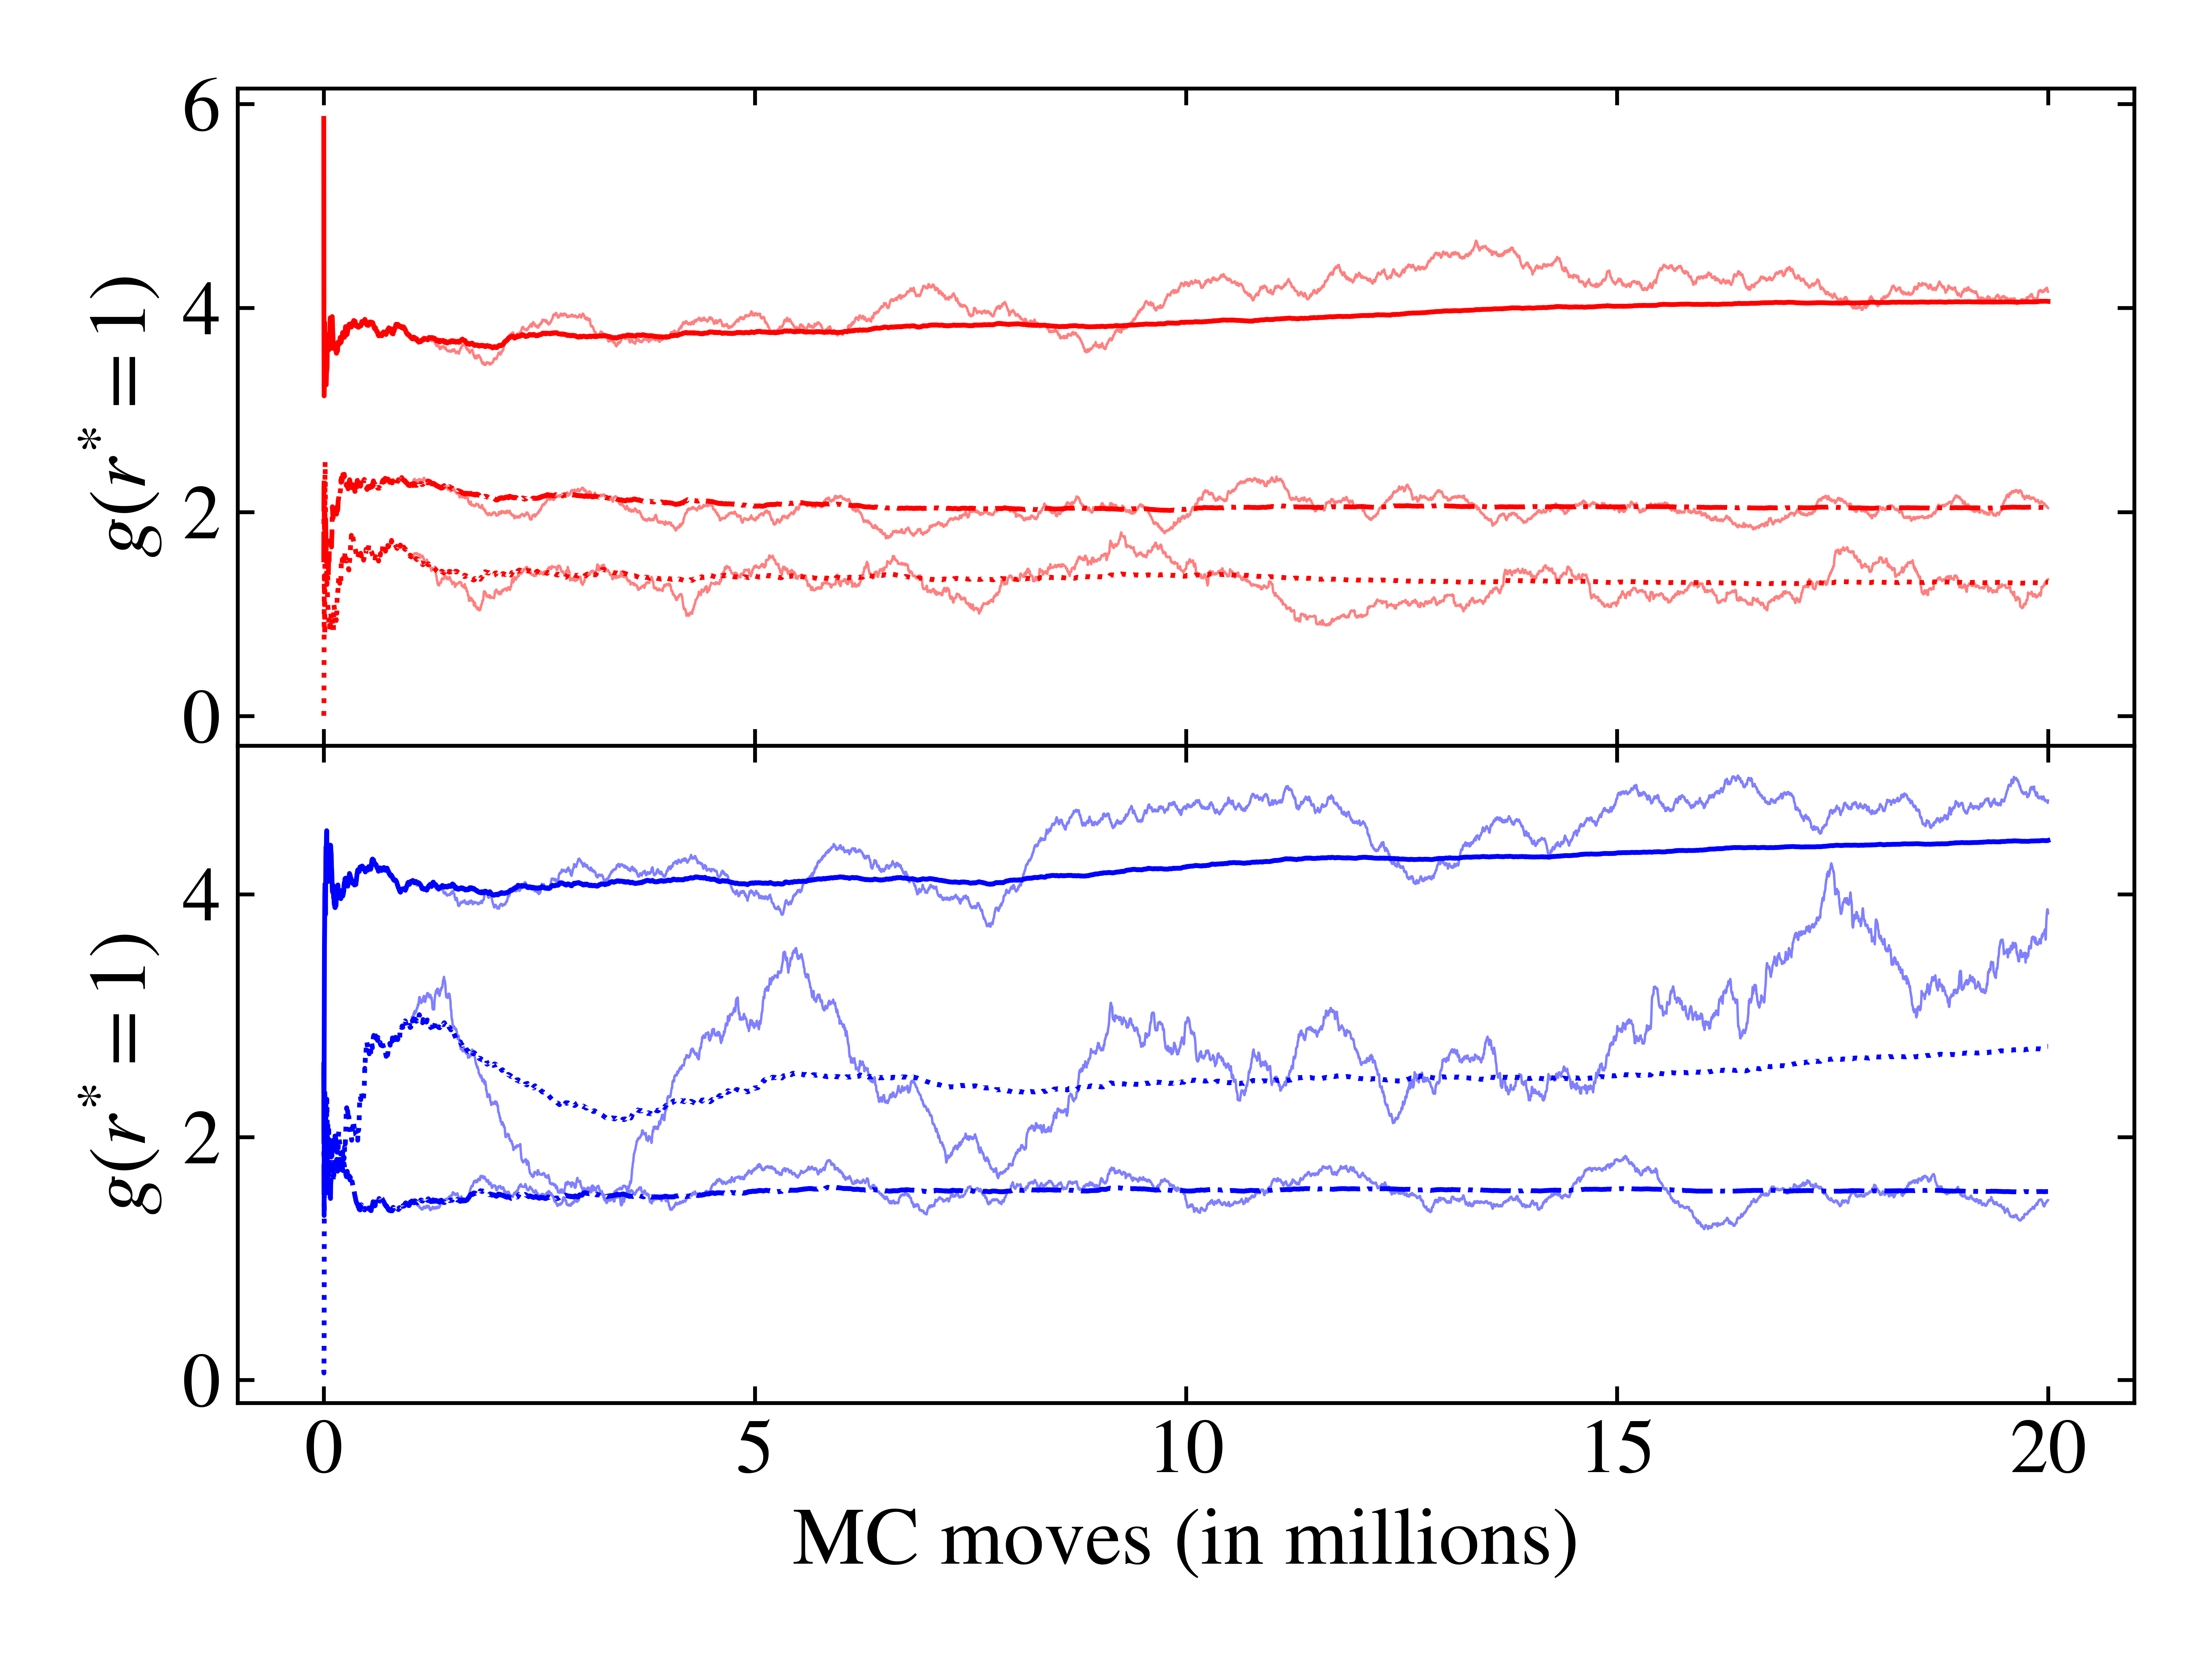
\includegraphics[width=\linewidth]{figures/convergence/gAtSigma_convergence.png}
	\caption{Typical convergence and fluctuation of the radial distribution function, $g(r^{*})$ evaluated at $r^{*}=1$. The smoother, darker lines show the variation of the cumulative average with increasing numbers of MC moves and are plotted for densities $\rho^{*} = 0.3, 0.8, 1.3$ represented by dotted, dash-dot, solid lines respectively. The lighter, jagged lines at any given point give a values of $g(r^{*}=1)$ averaged over the preceding 1 million MC moves. These are shown for isotherms $T^{*} = 0.75, 1.5$ represented by blue and red lines respectively. 
	}
	\label{fig:convergence}
\end{figure}

Graphs showing the convergence of the radial distribution function evaluated at $r^{*}=1$ and the fluctuation of a moving average over a fixed number of configurations for densities $\rho{}^{*}=0.3, 0.8, 1.3$ along isotherms $T^{*} = 0.75, 1.5$ are given in figure \ref{fig:convergence}. Ideally, we would have investigated the convergences of $u^{*}$ and $p^{*}$ however this would have required unduly amounts of computation time and the convergence $g(r^{*}=1)$ was chosen as a proxy for measuring the convergence of $g(r^{*})$ and thus $u^{*}$ and $p^{*}$.
These convergences are shown after the system had been equilibrated from its initial FCC configuration over \num{20e6} moves.
Along the isotherm $T^{*}=1.5$ the two lower density systems, $\rho{}^{*}=0.3, 0.8$, are observed to converge quite quickly, over approximately \num{2.5e6} moves with fluctuations of approximately $\pm{}10\%, 15\%$ respectively over the remaining moves. The system at $\rho{}^{*}=1.3$ seems to have initially converged quickly much like the lower density systems before starting to slowly rise after approximately \num{8e6} moves, evidenced by the fluctuations being distributed mostly around and then above the cumulative average in the two regions.
A similar trend is present in the system at $\rho{}^{*}=1.3$ along the isotherm $T^{*}=0.75$. Thus $g(r^{*}=1)$ is most likely underestimated in our high-density systems which, if it extends to $g(r^{*})$ for all $r^{*}$.
Convergence of the system at $T^{*}=0.75$, $\rho{}^{*}=0.8$ comparable to convergence at the same density along the higher isotherm, occurring over approximately \num{2.5e6} moves with fluctuations of $\pm{}10\%$.
Convergence of the system at $T^{*}=0.75$, $\rho{}^{*}=0.3$ shows qualitative characteristics not present in any of the other systems. First, the convergence of $g(r^{*}=1)$ displays some oscillatory behaviour which appears to stop at \num{10e6} moves. Fluctuations are then present fairly close to the cumulative average until \num{15e6} moves at which point $g(r^{*}=1)$ starts to increase. Without further investigation we are unable to comment on whether this increase continues past \num{20e6} moves. Thirdly, it is noted that $g(r^{*}=1)$ for $\rho{}^{*}=0.3$ converges to a higher value than for $\rho{}^{*}=0.8$. Since $g(r^{*}=1)$ can be interpreted as a measure of the likelihood of finding a particle a distance $r^{*}=1$ away from a reference particle, this would seemingly imply that particles in the lower density state are more tightly packed than particles in the higher density state.
The trend of systems at very high densities being harder to converge has been shown by other workers \cite{WoodParker}.

\begin{figure}
	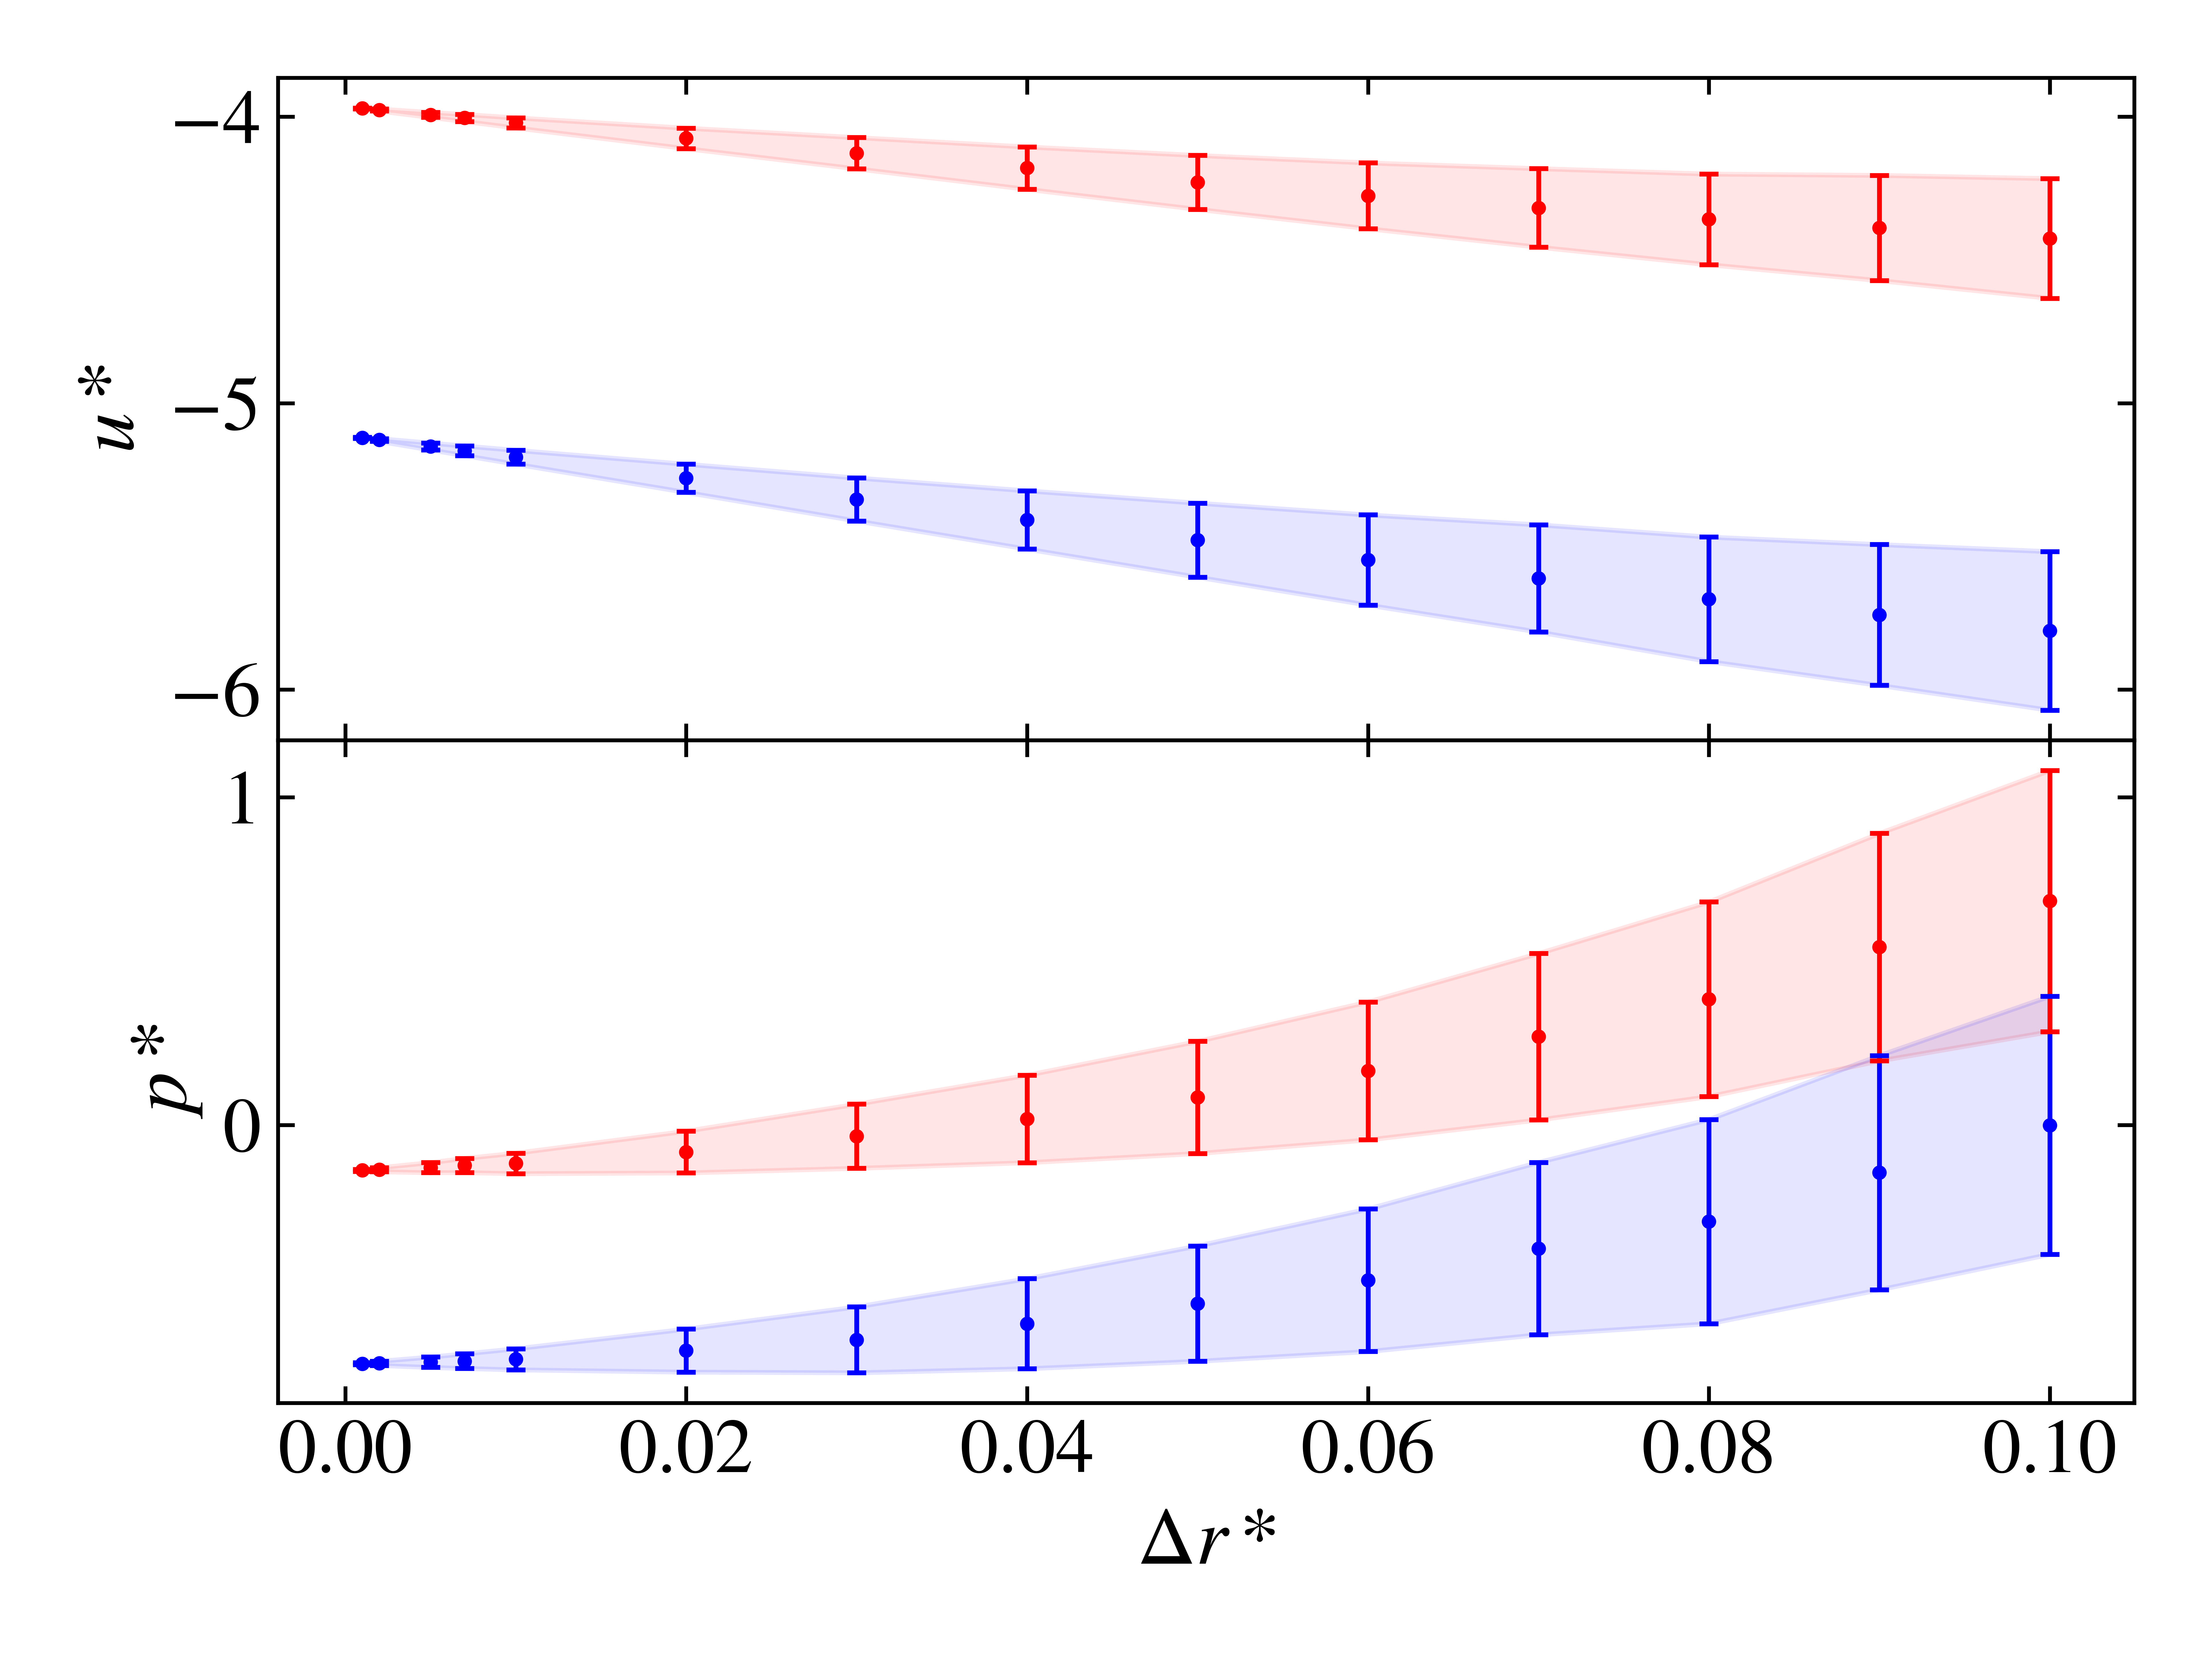
\includegraphics[width=\linewidth]{figures/binWidth/BWFeffect.png}
	\caption{Excess energy per particle, $u^{*}$, and excess pressure, $p^{*}$, against step-size $\Delta{}r^{*}$ (see discussion regarding equations \ref{eq:energy}, \ref{eq:pressure} in section \ref{s:methods}) evaluated for a system of density $\rho{}^{*}=0.6$ along isotherms $T^{*}=0.75, 1.5$ represented by blue and red markers respectively. Error bars show the standard error of the mean. Blue and red shaded areas are drawn to illustrate the increase in standard error with increasing step-size.}
	\label{fig:BWF}
\end{figure}


The step-size, $\Delta{}r^{*}$, in the numerical calculation of equations \ref{eq:energy} and \ref{eq:pressure} is a quantity of interest and importance. The closer $\Delta{}r^{*}$ to being infinitesimal, the closer our Riemann sum approximation is to evaluating the actual integral, leading to a more accurate result. However, the cost to decreasing $\Delta{}r^{*}$ is that the number of steps over which we evolve our systems must increase in order to maintain convergence, leading to prohibitive computation times at very small $\Delta{}r^{*}$. In order to explore the effect varying $\Delta{}r^{*}$ has on our results, we calculated $u^{*}$ and $p^{*}$ for systems of density $\rho{}^{*}=0.6$ along isotherms $T^{*}=0.75, 1.5$ at fourteen step-sizes ranging from \num{0.001} to \num{0.1}. This is shown in figure \ref{fig:BWF}. $u^{*}$ and $p^{*}$ are observed to decrease and increase respectively with increasing $\Delta{}r^{*}$. The standard errors of $u^{*}$ and $p^{*}$ both increase with $\Delta{}r^{*}$. A step size of \num{0.02} was chosen so that computations could be completed in a reasonable amount of time, corresponding to an approximate \num{3}\% (percentage) decrease in $u^{*}$ and a \num{0.05} (absolute) increase in $p^{*}$ along both isotherms. We do not account for these effects in our results - further investigation into the temperature and density dependences of this effect would need to be investigated in order to do so.


The accuracy of our model and method were investigated by direct comparison to Monte Carlo results at liquid and vapour-like densities along isotherms $T^{*} = 0.85, 0.90$ published by the National Institute of Standards and Technology (NIST). NIST's results are for \num{500} particles whose LJ interaction had been truncated to $r_\text{c}^{*}=3$ with standard long range corrections applied to $u^{*}$ and $p^{*}$. NIST's systems were equilibrated over \num{5.0e7} moves and quantities calculated over \num{2.5e8} moves, i.e. by factors of \num{2.5} and \num{12.5} more than ours. The configuration sampling rate of NIST's computations is not specified \cite{NIST}
Figure \ref{fig:NIST_u} shows $u^{*}$ from our simulations and NIST's data. With the exception of a single system, our values of $u^{*}$ are consistently reduced by \num{2} to \num{3}\% when compared the NIST data. This could be entirely attributed to the approximate \num{3}\% decrease found due to the Riemann sum approximation made in computing $u^{*}$ but this would need to be investigated further.
Figure \ref{fig:NIST_p} shows $p^{*}$ from our simulations and NIST's data. At vapour-like densities the absolute difference between our data and NIST's, $|\Delta{}p^{*}|$ increases linearly by a visual inspection. Our $p^{*}$ are observed to reduce below \num{0} with increasing density in this regime whereas NIST's results increase linearly with density by a visual inspection. At liquid-like densities, $\Delta{}p^{*}$ remains approximately constant at a value of about \num{-0.5}. This can not be accounted for by the effect of our approximation of equation \ref{eq:pressure} - in fact, it would place our values above those of NIST.
We find similar $\Delta{}u^{*}$ and $\Delta{}p^{*}$ when we compare our simulation to the extensive molecular dynamics results of Johnson et al \cite{Johnson}.

Mandel et al found $p^{*}$ to be extremely sensitive to small errors in correlation functions such as $g(r^{*})$, much more so than the pressure \cite{MandelEtAl}. If the errors in $u^{*}$ can be attributed largely to approximations made in its calculation then it is likely that some small error in the production of $g(r^{*})$ is the cause of the discrepancies found in $p^{*}$. This is supported by the breakdown observed when computing $g(r^{*})$ at low temperature and densities as discussed above and illustrated in the lower panel of figure \ref{fig:convergence}.

%\textbf{need to end discussion in a nicer way}


%\textit{The model and method were verified by direct comparison to Monte Carlo results at liquid and vapour-like densities along isotherms $T^{*}=0.85, 0.90$ published by United States' National Institute of Standard and Technology (NIST). NIST's results were for 500 particles whose Lennard-Jones interaction had been truncated to $3\sigma{}$ and standard long range corrections had been applied. Their systems were equilibrated for $5.0\text{e}7$ moves and quantities calculated over $2.5\text{e}8$ moves. Figure \ref{fig:NIST_comparison} shows the configuration energy per particle, $u^*$, and virial pressure, $p^{*} = P - \rho{}kT$ for both our system and NIST's. Our results were obtained as described in section \ref{s:methods}. See appendix \ref{a:NIST} for the values and their associated uncertainties of NIST's and our simulations.}


\begin{figure}
	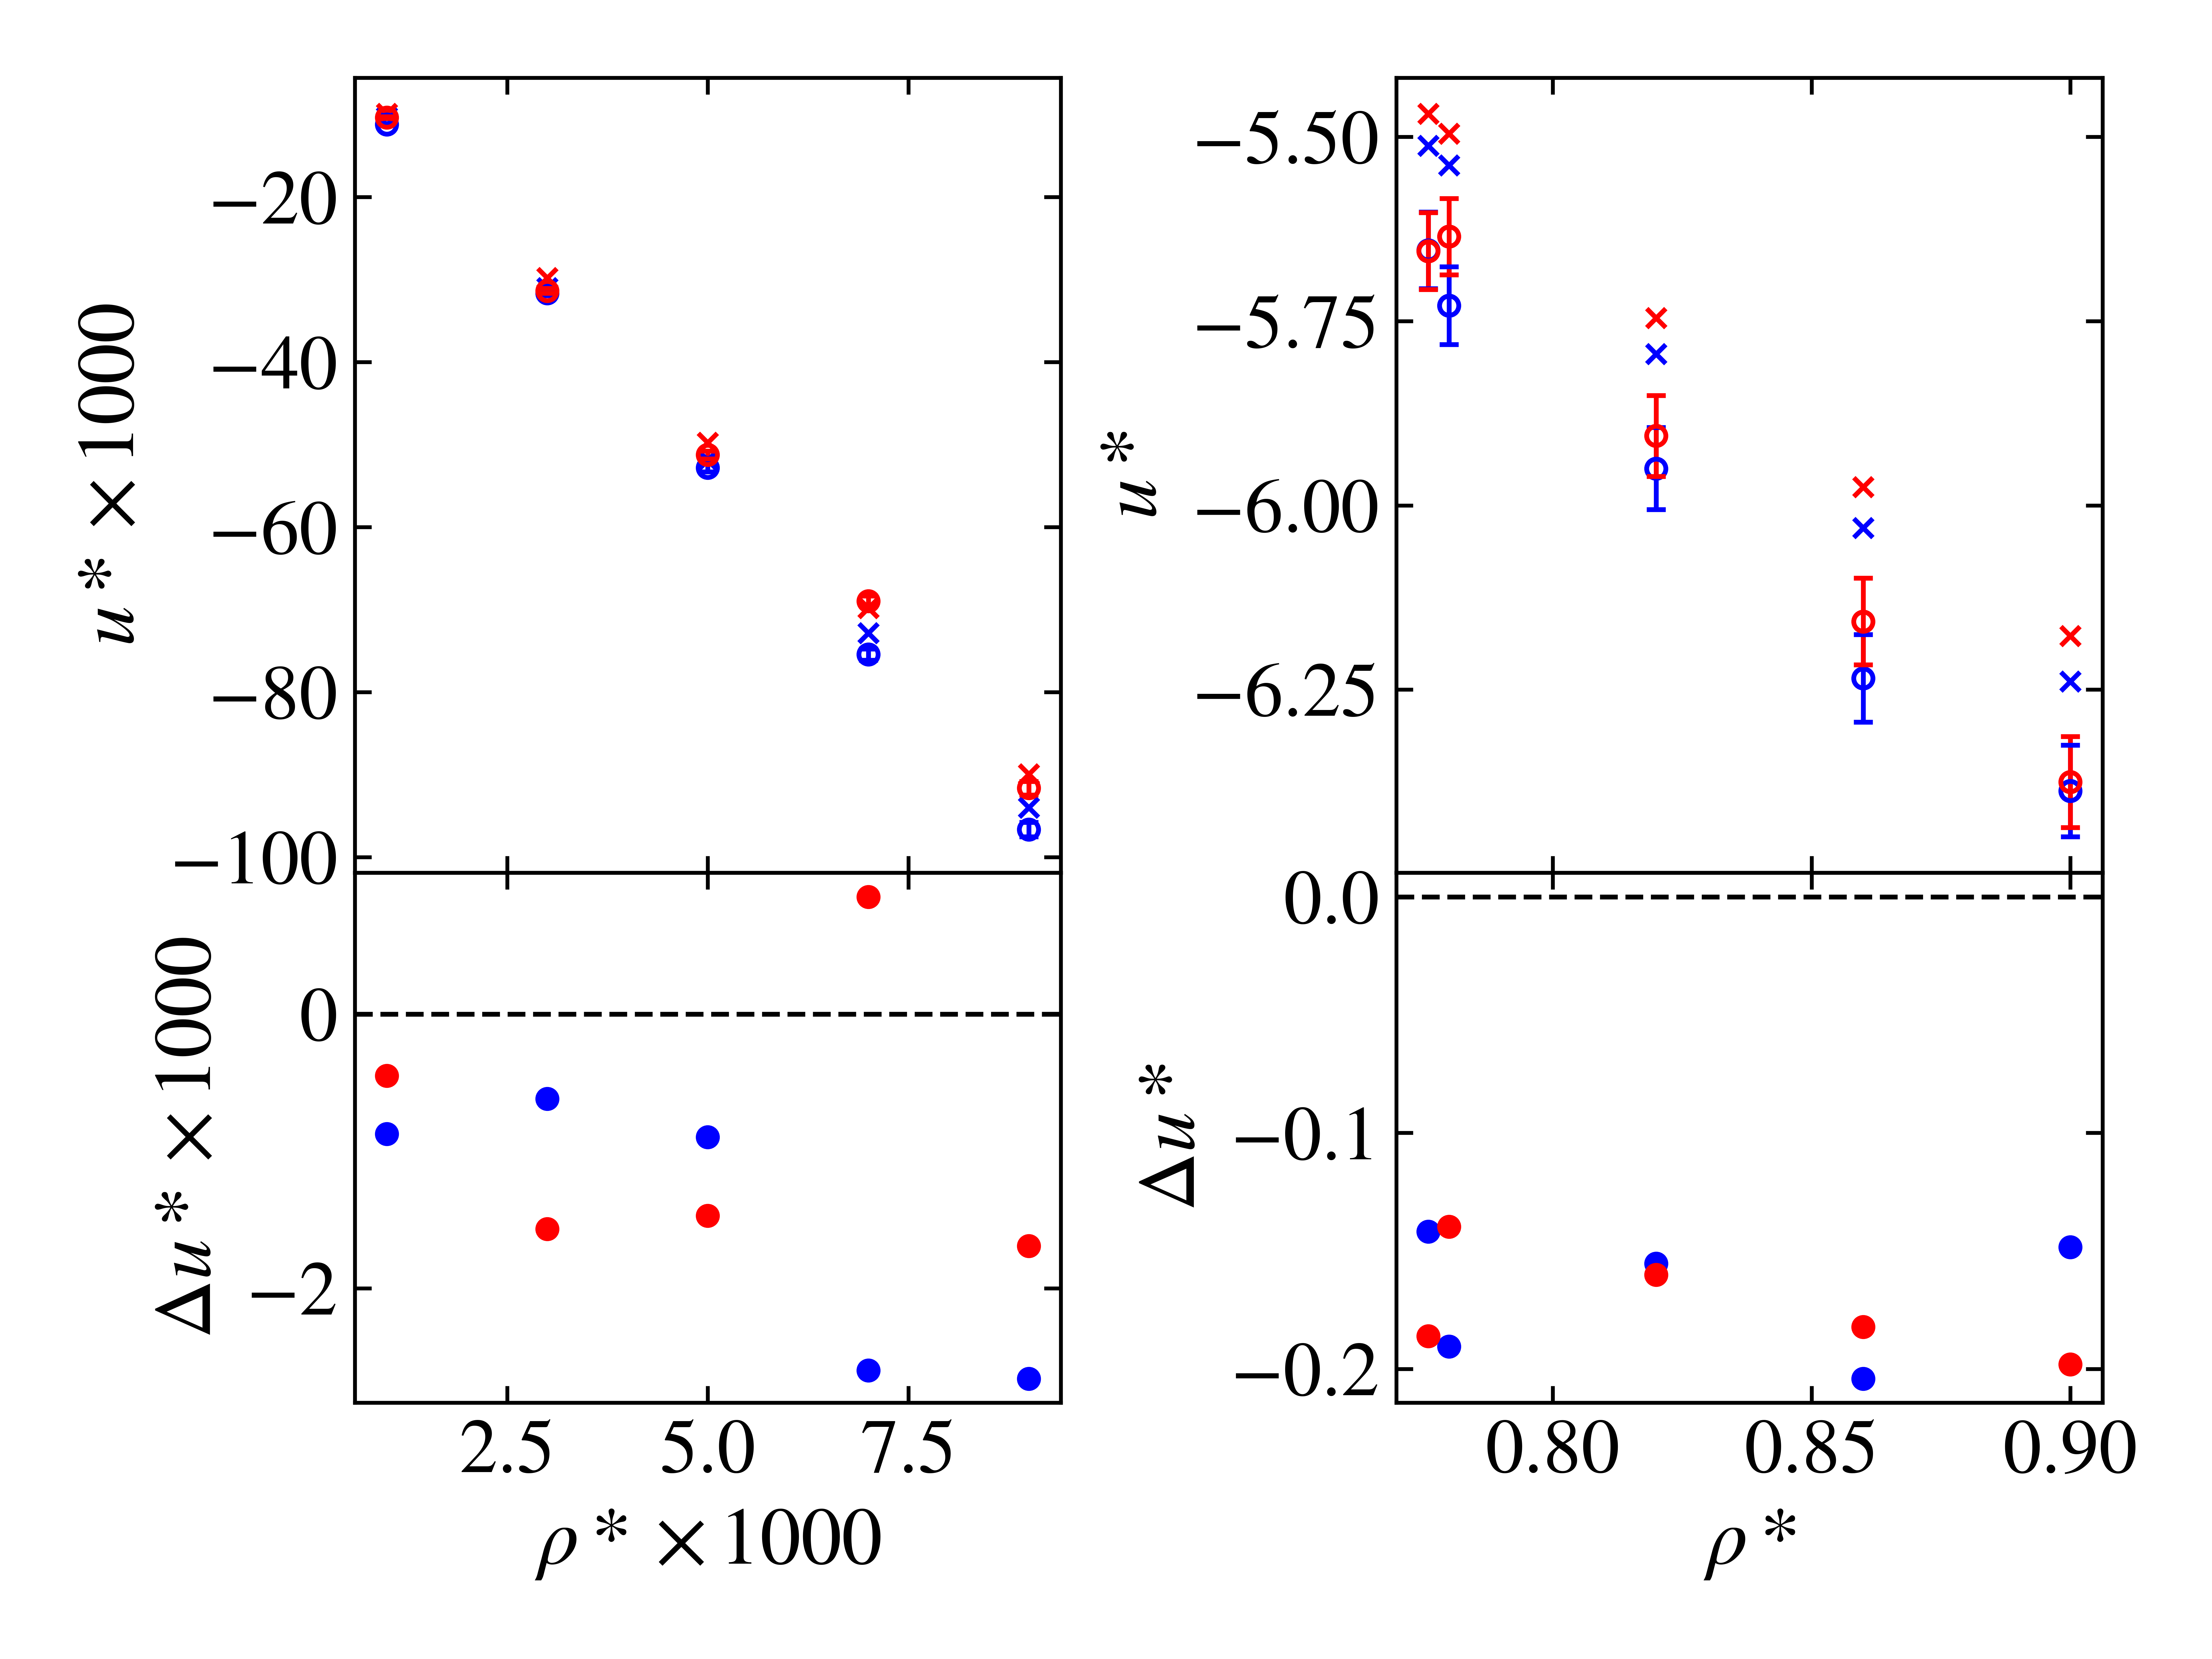
\includegraphics[width=\linewidth]{figures/NIST_comparison/NIST_u.png}
	\caption{Excess energy per particle, $u^{*}$, at vapour-like (upper-left panel) and liquid-like (upper-right panel) densities, $\rho{}^{*}$. Our MC results and those of the National Institute of Standards and Technology (NIST) are represented by unfilled circles and crosses respectively. Data is shown for isotherms $T^{*}=0.85, 0.90$ by blue and red markers respectively. Error bars for our MC data show the standard error of the mean. Error bars are not shown for NIST's data for visual clarity. The differences between our results and NIST's results, $\Delta{}u^{*} = u_\text{our}^{*} - u_\text{NIST}^{*}$ are shown in the lower panel. A dotted line has been added along $\Delta{}u^{*}=0$ for reference. Note that some values have been scaled by a factor of 1000.}
	\label{fig:NIST_u}
\end{figure}

\begin{figure}
	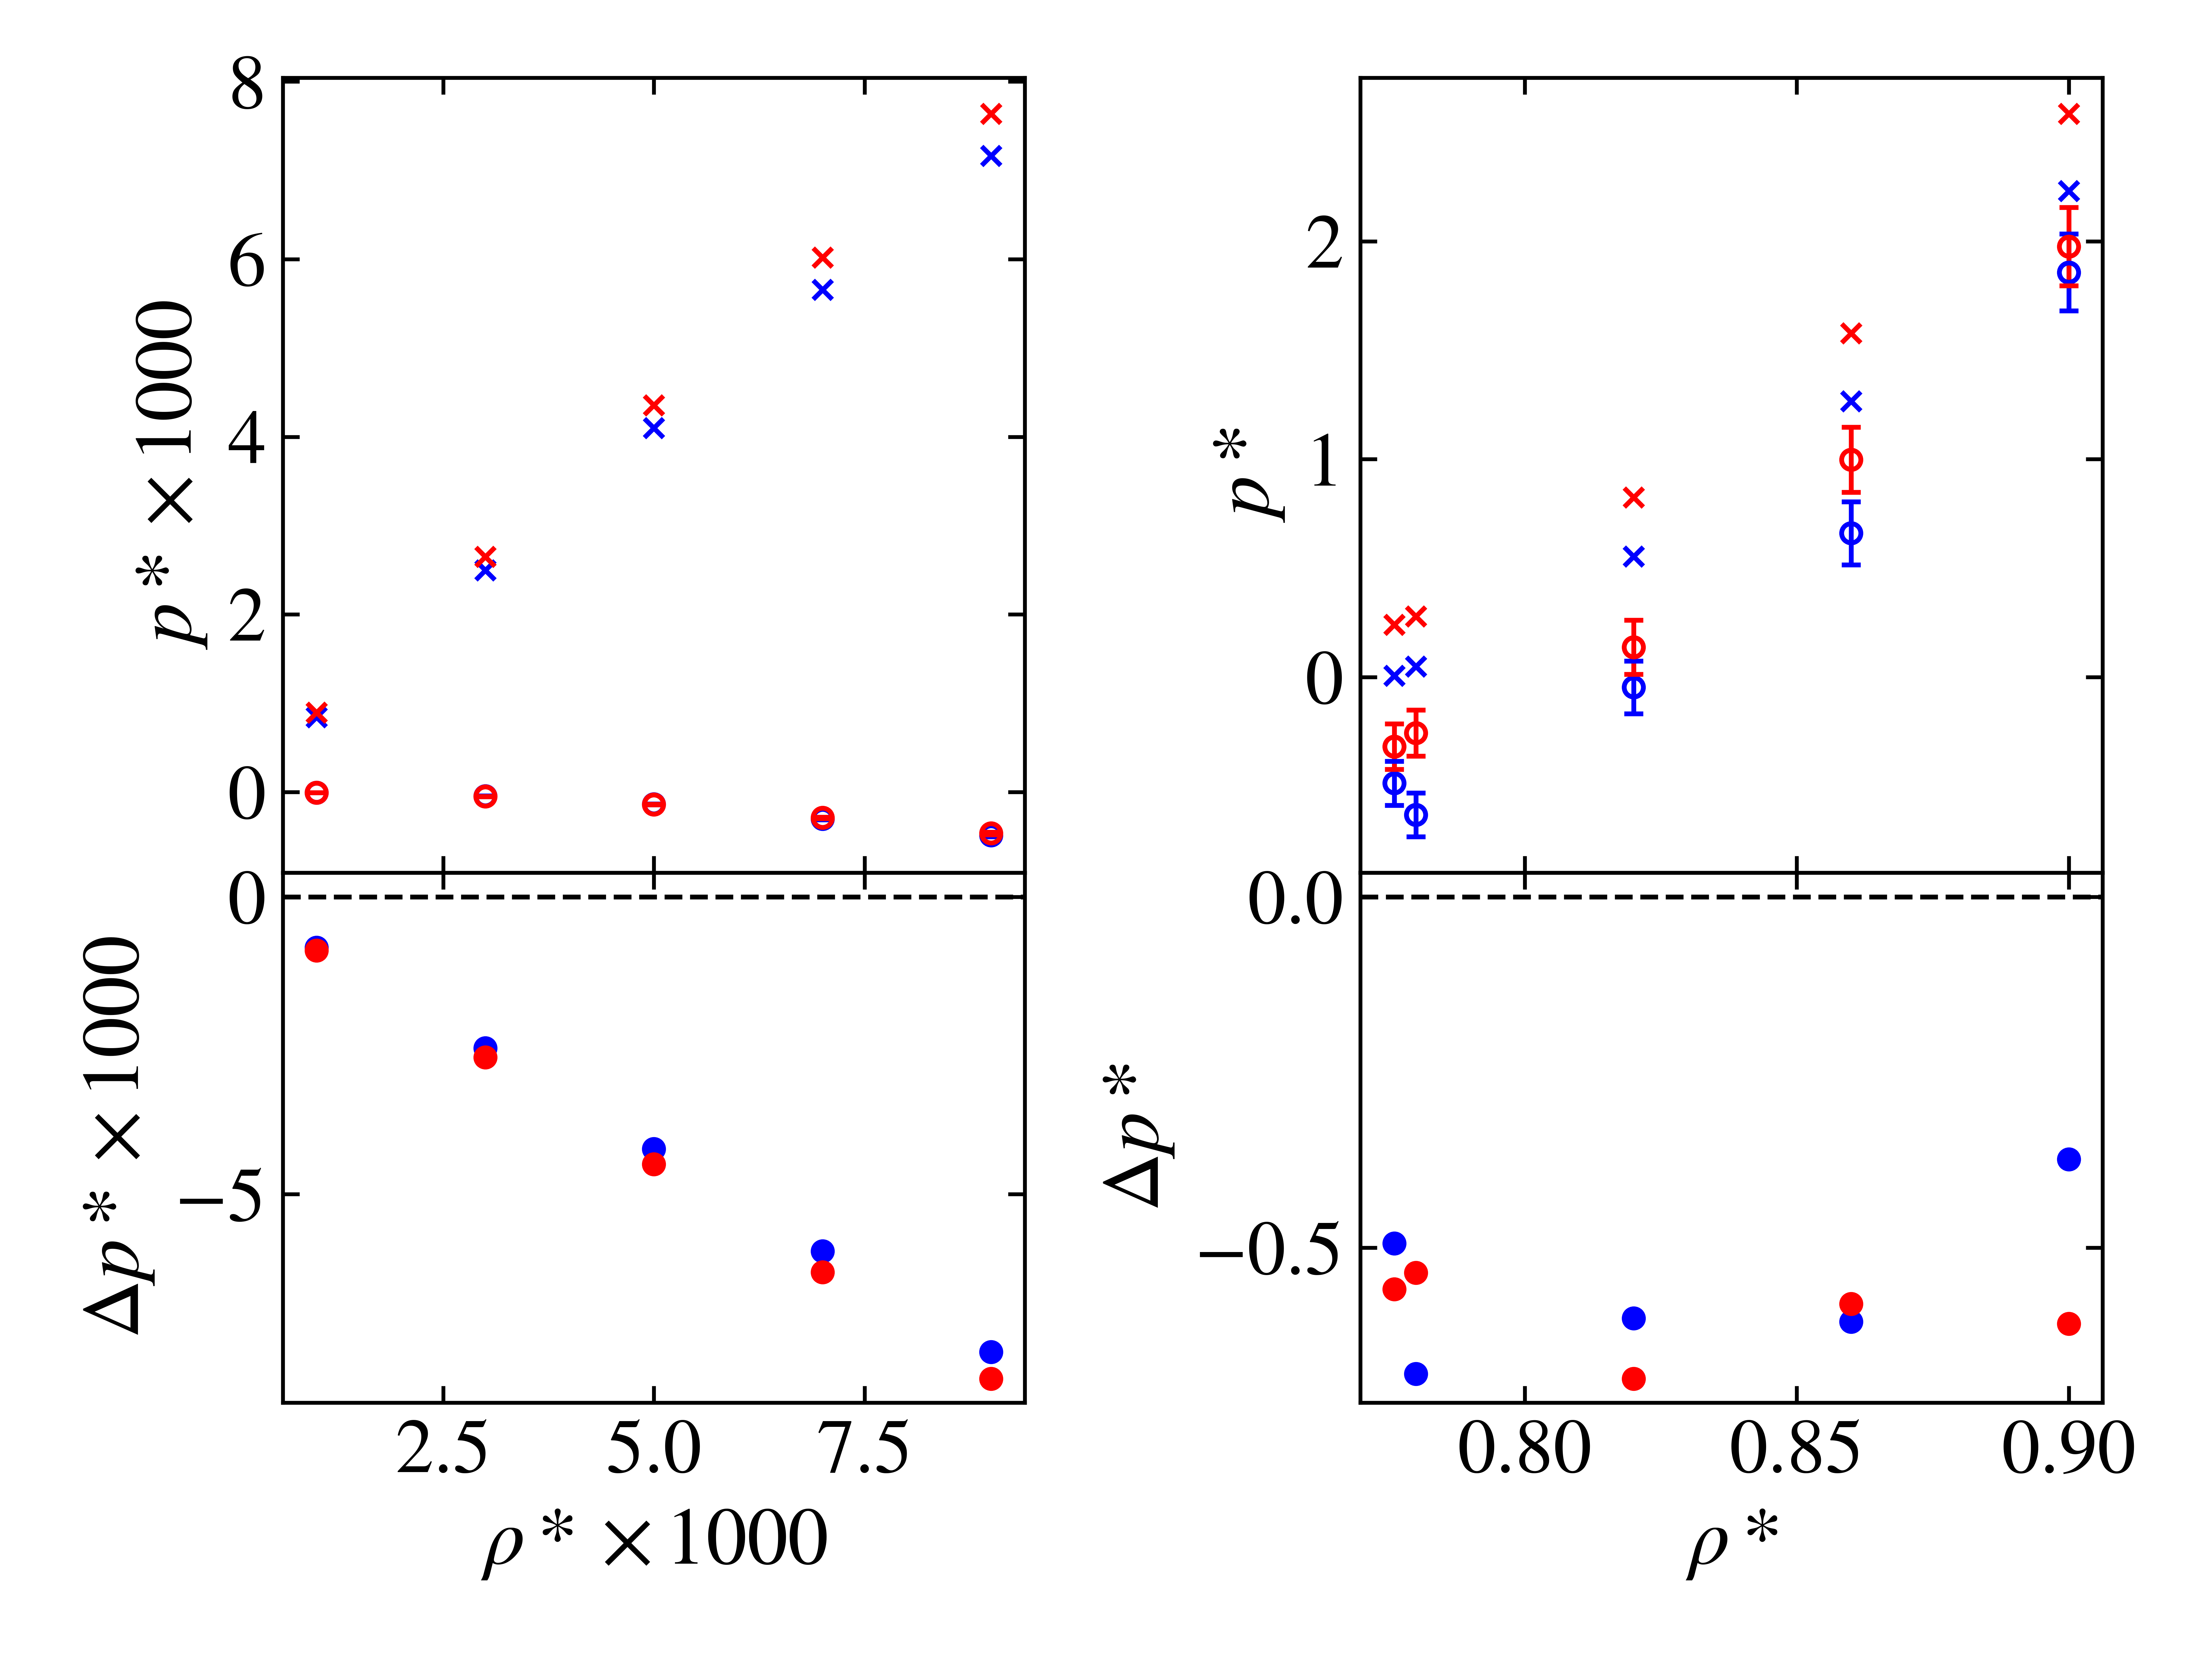
\includegraphics[width=\linewidth]{figures/NIST_comparison/NIST_p.png}
	\caption{Excess pressure, $p^{*}$, at vapour-like (upper-left panel) and liquid-like (upper-right panel) densities, $\rho{}^{*}$. Our MC results and those of the National Institute of Standards and Technology (NIST) are represented by unfilled circles and crosses respectively. Data is shown for isotherms $T^{*}=0.85, 0.90$ by blue and red markers respectively. Error bars for our MC data show the standard error of the mean. Error bars are not shown for NIST's data for visual clarity. The differences between our results and NIST's results, $\Delta{}p^{*} = p_\text{our}^{*} - p_\text{NIST}^{*}$ are shown in the lower panel. A dotted line has been added along $\Delta{}p^{*}=0$ for reference. Note that some values have been scaled by a factor of 1000.}
	\label{fig:NIST_p}
\end{figure}

%\section{Discussion} \label{s:analysis}
%\lipsum[1-15]



\section{Conclusions} \label{s:conclusions}
This work presented Monte Carlo results for a thousand three-dimensional Lennard-Jones particles in a cubic container. Excess energy and pressure were reported for twenty-four reduced densities between \num{0.05} and \num{1.50} along reduced temperatures \num{0.75}, \num{1.00}, \num{1.25}, \num{1.50}. The shapes of our density dependence of the excess energy and pressure are found to be consistent with literature with the exception of the excess energy at low temperatures and densities which displays erratic behaviour. We suggest that this is due to small errors in the evaluation of the radial distribution function for these systems. We find a significant dependence on the step-size chosen when numerically calculating the integral expressions for the excess energy and pressure. With further investigation this dependence could potentially be accounted for in results, allowing for accurate excess energy calculations even with relatively small numbers of Monte Carlo moves. The excess energy and pressure of dilute Lennard-Jones particles are found to be fairly well approximated by an ideal gas. Vapour, liquid, and solid states are observed in our systems and typical radial distribution functions presented.

\begin{thebibliography}{}

%\bibitem{ref01} A. N. Other, Title of the Book, edition, publishers, place of publication (year of publication), p. 123.   % example reference



\bibitem{MC} N. Metropolis, et al., Equation of State Calculations by Fast Computing Machines, J. Chem. Phys. 21, 1087 (1953), doi:10.1063/1.1699114

\bibitem{CompSimLiq} M. P. Allen, D. J. Tildesley, Computer Simulation of Liquids, 2nd, Oxford University Press, Oxford (2017), chs. 1, 4

\bibitem{Frenkel} D. Frenkel, Entropy-driven phase transitions, Physica A 263, 26-38 (1999), doi:10.1016/S0378-4371(98)00501-9

\bibitem{Hansen2} J. P. Hansen, Phase Transition of the Lennard-Jones System. II. High-Temperature Limit, Phys. Rev. A 2, 221 (1970), doi:10.1103/PhysRevA.2.221

\bibitem{SimpleLiquids} J. P. Hansen, I. R. McDonald, Theory of Simple Liquids, 3rd, Academic Press, Massachusetts (2006) ch. 1

\bibitem{WoodParker} W. W. Wood, F. R. Parker, Monte Carlo Equation of State of Molecules Interacting with the Lennard-Jones Potential. I. A Supercritical Isotherm at about Twice the Critical Temperature, J. Chem. Phys. 27, 720 (1957), doi:10.1063/1.1743822

\bibitem{NIST} Published data for testing codes: Lennard-Jones Fluid Properties, National Institute of Standards and Technology, accessed 17 Feb 2020, available at: https://www.nist.gov/mml/csd/chemical-informatics-research-group/lennard-jones-fluid-properties

\bibitem{Johnson} J. K. Johnson, The Lennard-Jones equation of state revisited , Mol. Phys. 78:3, 591-618 (1993), doi:10.1080/00268979300100411

\bibitem{errors}I. G. Hughes, T. P. A Hase, Measurements and their Uncertainties A Practical Guide to Modern Error Analysis, 1st, Oxford University Press, Oxford (2010)

\bibitem{HansenVerlet1} J. P. Hansen, L. Verlet, Phase Transitions of the Lennard-Jones System, Phys. Rev. 184, 151 (1969), doi:10.1103/PhysRev.184.151

\bibitem{Ree} F. H. Ree, Analytic representation of thermodynamic data for the Lennard-Jones fluid, J. Chem. Phys. 73, 5401 (1980), doi:10.1063/1.439940

\bibitem{MandelEtAl} F. Mandel, et al., Numerical Solutions of the Percus-Yevick Equation for the Lennard-Jones (6-12) and Hard-Sphere Potentials, J. Chem. Phys. 52, 3315 (1970), doi:10.1063/1.1673491


\end{thebibliography} 

%\clearpage
%\appendix
%\section{Error Analysis} \label{a:errors}
%All propagation of errors is performed as outlined in \cite{errors}.
%
%\clearpage
%\section{Comparison to NIST data} \label{a:NIST}
%
%
%% Please add the following required packages to your document preamble:
%% \usepackage{booktabs}
%% \usepackage{multirow}
%% \usepackage{graphicx}
%\begin{table}[]
%	\resizebox{\textwidth}{!}{%
%		\begin{tabular}{@{}rrrrrrrrrr@{}}
%			\toprule
%			$T^*$                  & $\rho{}^*$ & $U_\text{NIST}^*$ & $\pm$    & $U_\text{ours}^*$ & $\pm$   & $p_\text{NIST}^*$ & $\pm$    & $p_\text{ours}^*$ & $\pm$   \\ \midrule
%			\multirow{10}{*}{0.85} & 1.00E-3    & -1.0317E-2       & 2.34E-5 & -9.968E-3         & 9.17E-5 & 8.4402E-4        & 4.66E-8 & -5.288E-6         & 1.72E-7 \\
%			& 3.00E-3    & -3.1019E-2       & 5.91E-5 & -3.156E-2         & 2.87E-4 & 2.4965E-3        & 4.99E-7 & -6.121E-5         & 1.48E-6 \\
%			& 5.00E-3   & -5.1901E-2       & 7.53E-5 & -5.485E-2         & 5 .07E-4 & 4.1003E-3        & 5.05E-7 & -1.472E-4         & 4.75E-6 \\
%			& 7.00E-3   & -7.2834E-2       & 1.34E-4 & -7.499E-2         & 6.87E-4 & 5.6565E-3        & 7.96E-7 & -2.854E-4         & 8.98E-6 \\
%			& 9.00E-3   & -9.3973E-2       & 1.29E-4 & -9.863E-2         & 9.18E-4 & 7.1641E-3        & 2.24E-6 & -4.568E-4         & 1.51E-5 \\
%			& 7.76E-1   & -5.5121       & 4.55E-4 & -5.623            & 5.21E-2 & 6.7714E-3        & 1.77E-3 & -5.577E-1         & 9.91E-2 \\
%			& 7.80E-1   & -5.5386       & 7.26E-4 & -5.611            & 5.14E-2 & 4.7924E-2        & 3.18E-3 & -6.311E-1         & 9.88E-2 \\
%			& 8.20E-1   & -5.7947       & 6.03E-4 & -5.908            & 5.59E-2 & 5.5355E-1        & 4.13E-3 & 2.588E-1          & 1.25E-1 \\
%			& 8.60E-1   & -6.0305       & 2.38E-3 & -6.175            & 5.87E-2 & 1.2660        & 1.36E-2 & 4.973E-1          & 1.41E-1 \\
%			& 9.00E-1   & -6.2391       & 5.27E-3 & -6.346            & 6.17E-2 & 2.2314        & 2.72E-2 & 1.823             & 1.75E-1 \\ \cmidrule(lr){1-10}
%			\multirow{10}{*}{0.90} & 1.00E-3   & -9.9165E-3       & 1.89E-5 & -9.989E-3         & 9.05E-5 & 8.9429E-4        & 2.48E-8 & -6.475E-6         & 1.76E-7 \\
%			& 3.00E-3   & -2.9787E-2       & 3.21E-5 & -3.065E-2         & 2.79E-4 & 2.6485E-3        & 2.54E-7 & -4.368E-5         & 1.70E-6 \\
%			& 5.00E-3   & -4.9771E-2       & 3.80E-5 & -5.226E-2         & 4.75E-4 & 4.3569E-3        & 2.19E-7 & -1.426E-4         & 4.35E-6 \\
%			& 7.00E-3   & -6.9805E-2       & 7.66E-5 & 7.179E-2          & 6.50E-4 & 6.0193E-3        & 1.02E-6 & -3.075E-4         & 8.14E-6 \\
%			& 9.00E-3   & -8.9936E-2       & 2.44E-5 & -9.151E-2         & 8.33E-4 & 7.6363E-3        & 1.44E-6 & -4.295E-4         & 1.41E-5 \\
%			& 7.76E-1   & -5.4689       & 4.20E-4 & -5.615            & 5.21E-2 & 2.4056E-1        & 2.74E-3 & -2.486E-1         & 1.04E-1 \\
%			& 7.80E-1   & -5.4956       & 7.86E-4 & -5.627            & 5.20E-2 & 2.7851E-1        & 2.97E-3 & -2.576E-1         & 1.06E-1 \\
%			& 8.20E-1   & -5.7456       & 7.51E-4 & -5.870            & 5.53E-2 & 8.2386E-1        & 2.85E-3 & 2.921E-1          & 1.25E-1 \\
%			& 8.60E-1   & -5.9753       & 5.53E-4 & -6.130            & 5.89E-2 & 1.5781        & 3.29E-3 & 1.193             & 1.53E-1 \\
%			& 9.00E-1   & -6.1773       & 1.57E-3 & -6.312            & 6.14E-2 & 2.5848        & 9.54E-3 & 1.871             & 1.75E-1 \\ \bottomrule
%		\end{tabular}%
%	}
%\end{table}

\end{document}